\documentclass[hidelinks,12pt]{article}
\usepackage[utf8]{inputenc}
\usepackage[T1]{fontenc}
%\usepackage[french]{babel}
\usepackage{times}
\usepackage{hyperref}
\usepackage{graphicx}

\begin{document}

\title{Research project report}
\author{Bastien Nony, Alban Gossard\\
Institut National des Sciences Appliquées,\\
Toulouse,\\
\href{mailto:nony@etud.insa-toulouse.fr}{   \texttt{nony@etud.insa-toulouse.fr}}\\
\href{mailto:gossard@etud.insa-toulouse.fr}{   \texttt{gossard@etud.insa-toulouse.fr}}}
\date{\today}

\maketitle

\begin{abstract}
In this work we study surrogates problems for different types of modelling problem. The objective is to provide fast calculation for undetermined values. Beginning from physical equations such as Saint-Venant's, we add statistical formulas to determine the variability of the system.
\end{abstract}

\tableofcontents


\section*{Introduction}
\addcontentsline{toc}{section}{Introduction}



\section{Study of 1D model}

\subsection{Surrogate method : kriging}

We compute different surrogate using different initial sample size. These surrogates were computed using a least square strategy. Figure \ref{influence_init_size_method_surrogate_kriging} gives the simulations results for the surrogate. One can observe that we obtain almost the same resultats as the initial sample size is greater than 10. As we will explain in part \ref{}, the results are quite precise but we have no information about the standard deviation of this new model and its sensibility to the parameters. Computing a surrogate with a greater number of points is fundamental to get a quantification of the error.

\begin{figure}[!t]
\centering
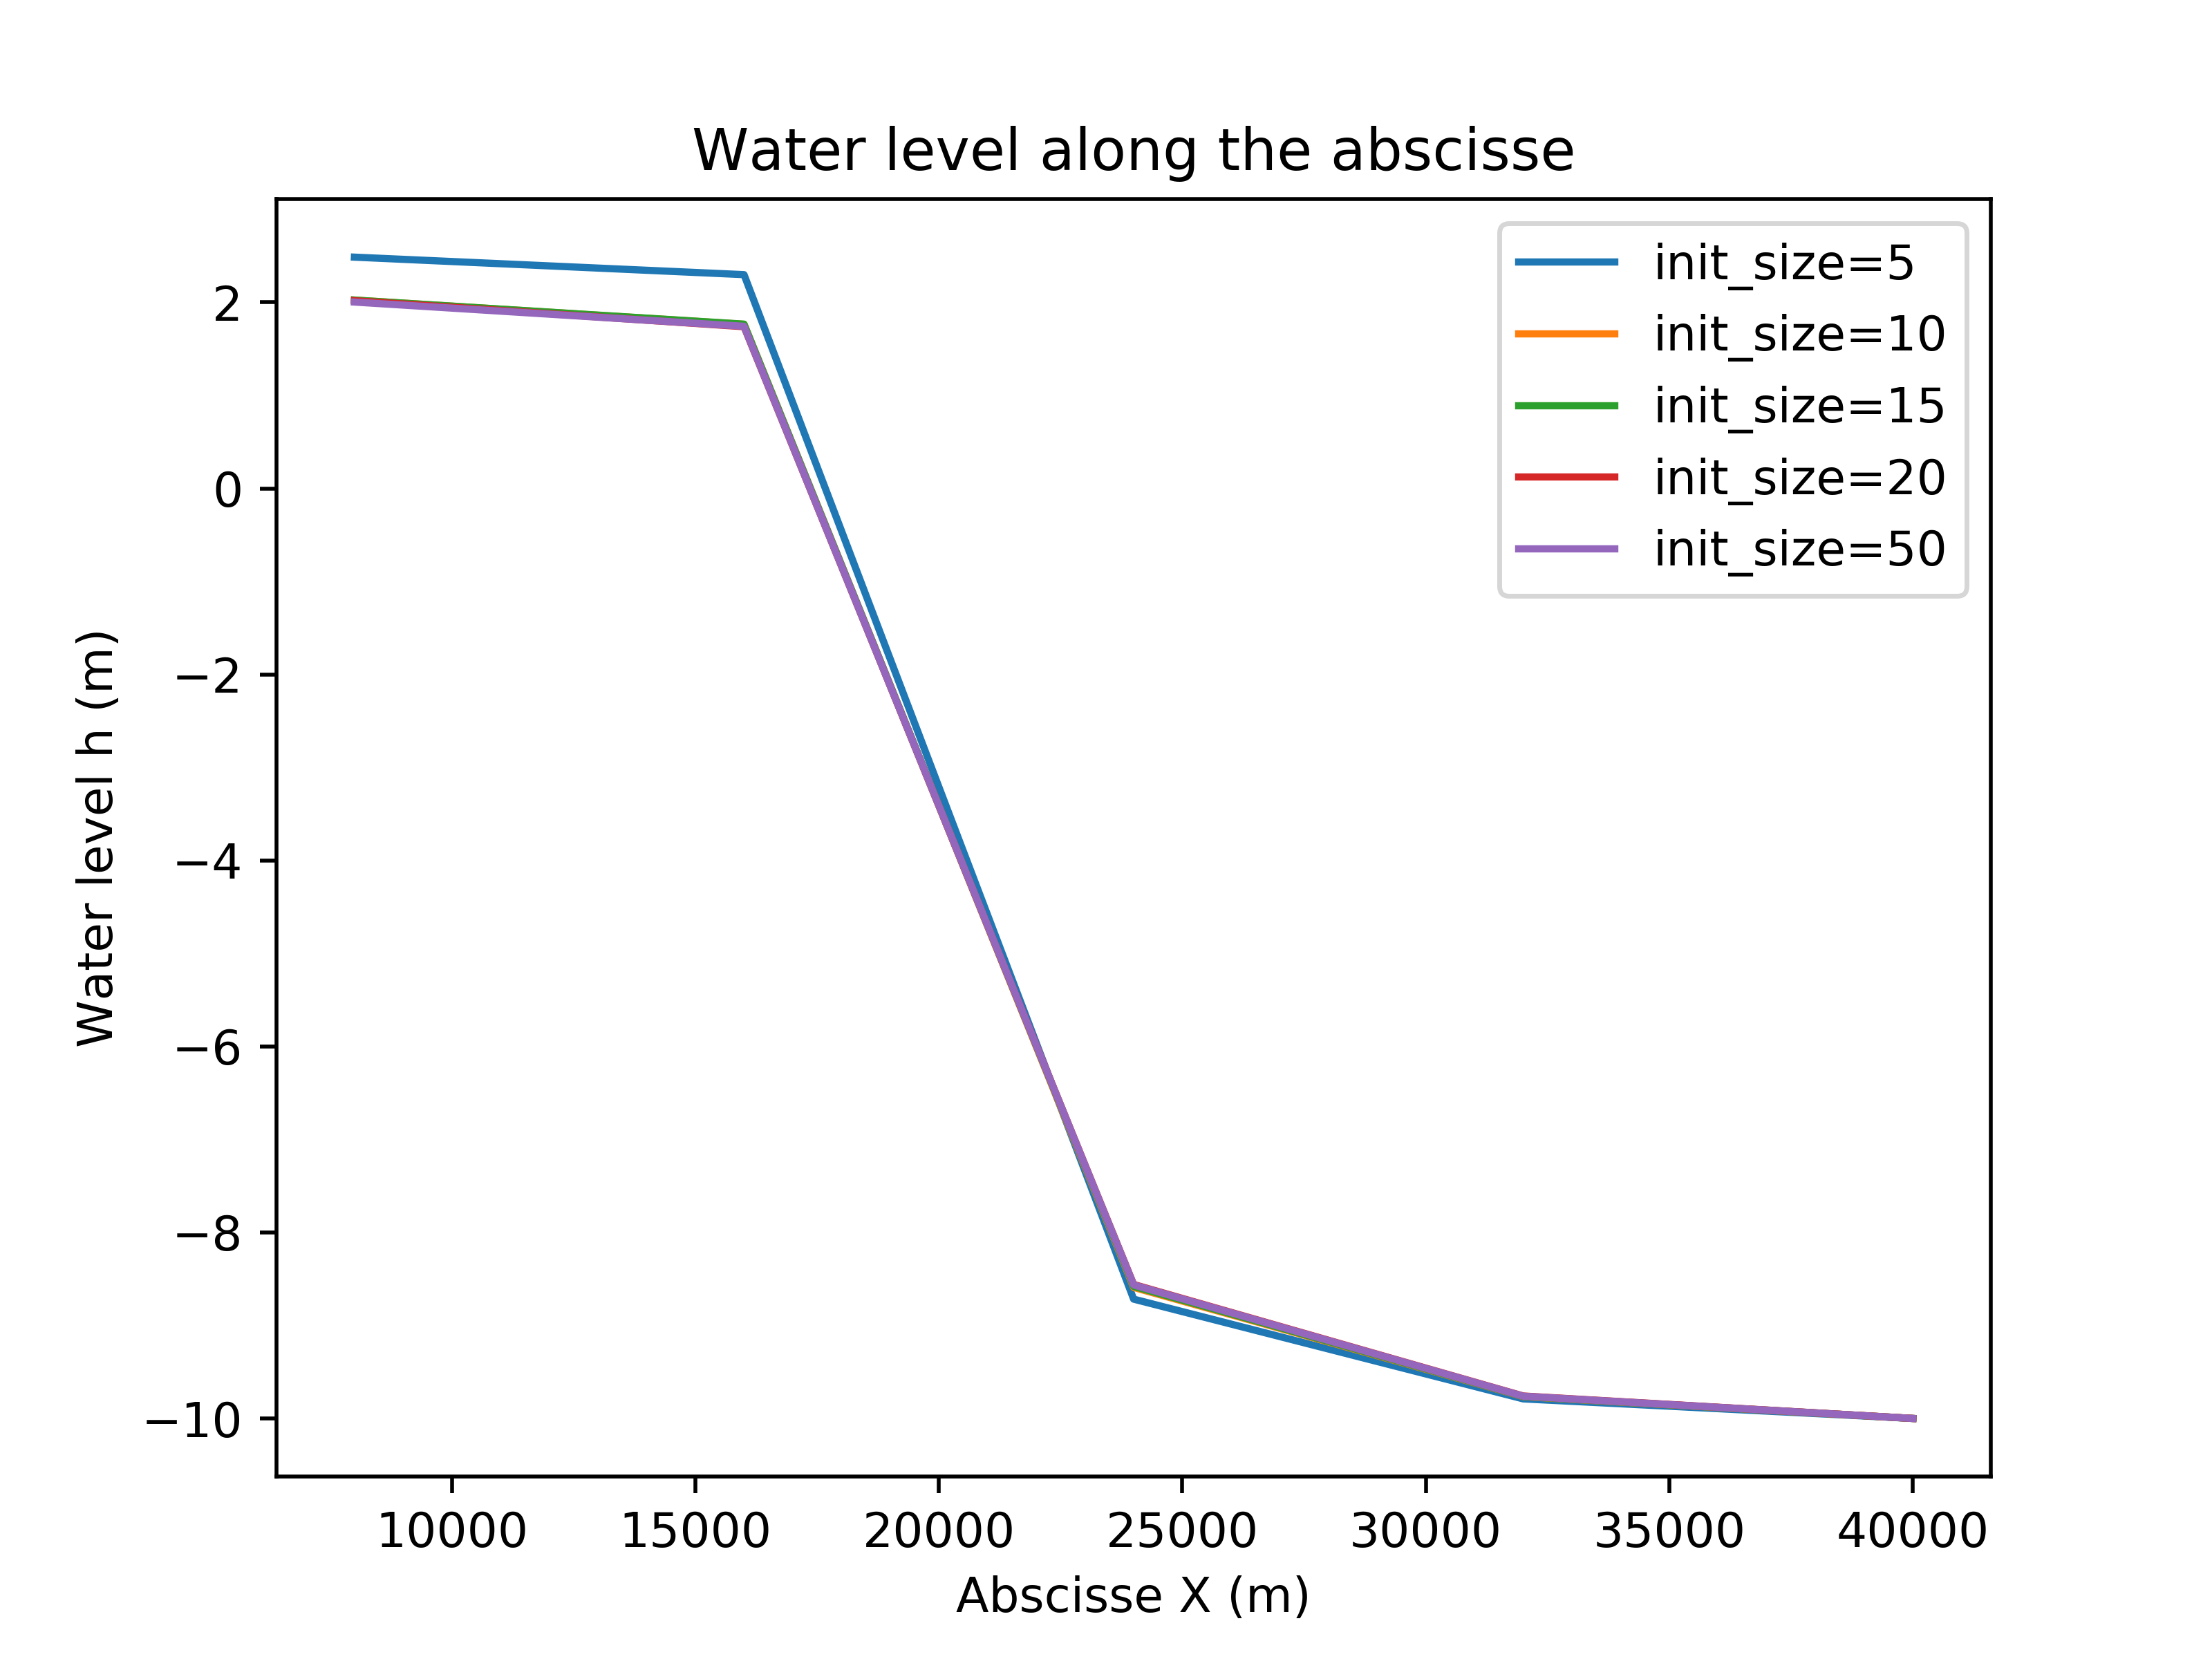
\includegraphics[width=0.8\textwidth]{images/influence_init_size_method_surrogate_kriging.png}
\caption{Water level along the abscisse for simulations with different initial sample size using kriging method for surrogate computing.}
\label{influence_init_size_method_surrogate_kriging}
\end{figure}

\subsection{Surrogate method : pc}

\begin{figure}[!t]
\centering
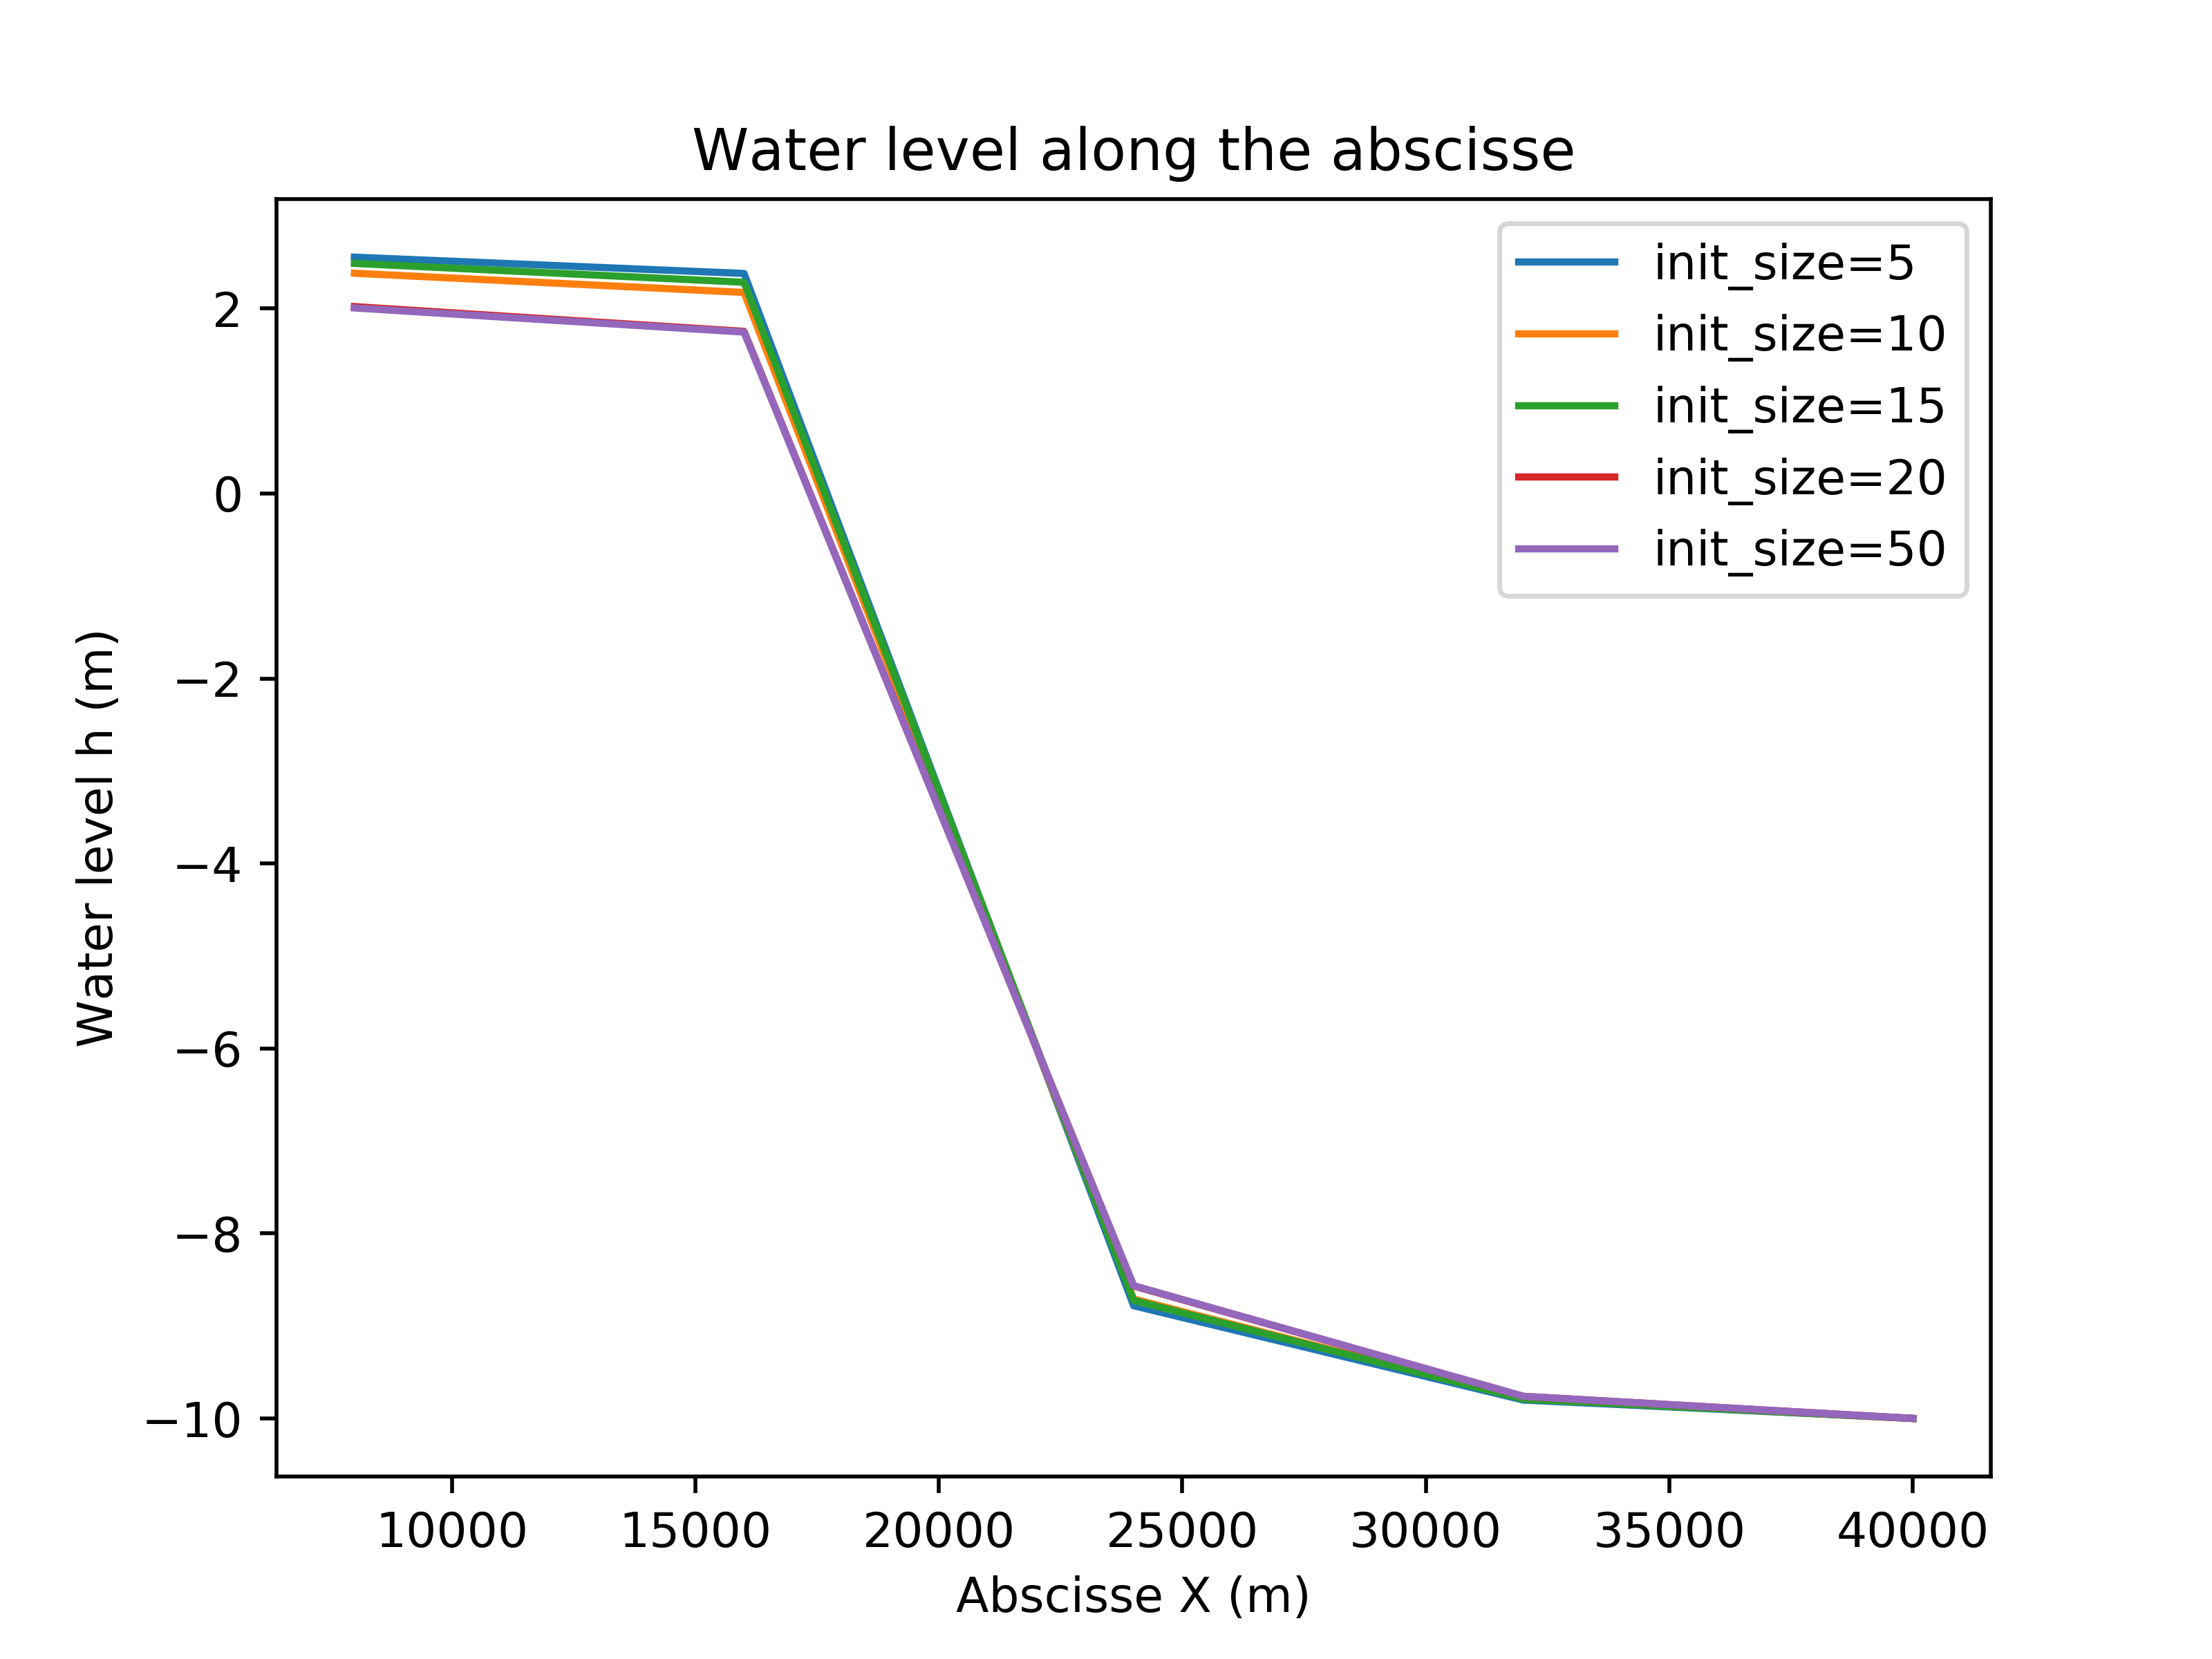
\includegraphics[width=0.8\textwidth]{images/influence_init_size_method_surrogate_pc.png}
\caption{Water level along the abscisse for simulations with different initial sample size using pc method for surrogate computing.}
\label{influence_init_size_method_surrogate_kriging}
\end{figure}


\end{document}

